\section{W-mass}
\label{sec:w-mass}
With the finished calibration, the mass of the W-boson can now be measured. This is done using a the Jacobi peak of the electron transverse momentum distribution.
In order to determine the W-mass, we use a data set of actual ATLAS data containing $W \rightarrow e\nu$ events,
as well as several simulated data sets also containing $W \rightarrow e\nu$ events. 
There is also a $Z^0 \rightarrow e^+e^-$ data set to check the validity of the previous calibration.
Finally there are data sets for QCD- and non-QCD background events.

\subsection{Electron Calibration Verification}
    \label{sec:calibration_verification}
    \begin{figure}[H]
        \centering
        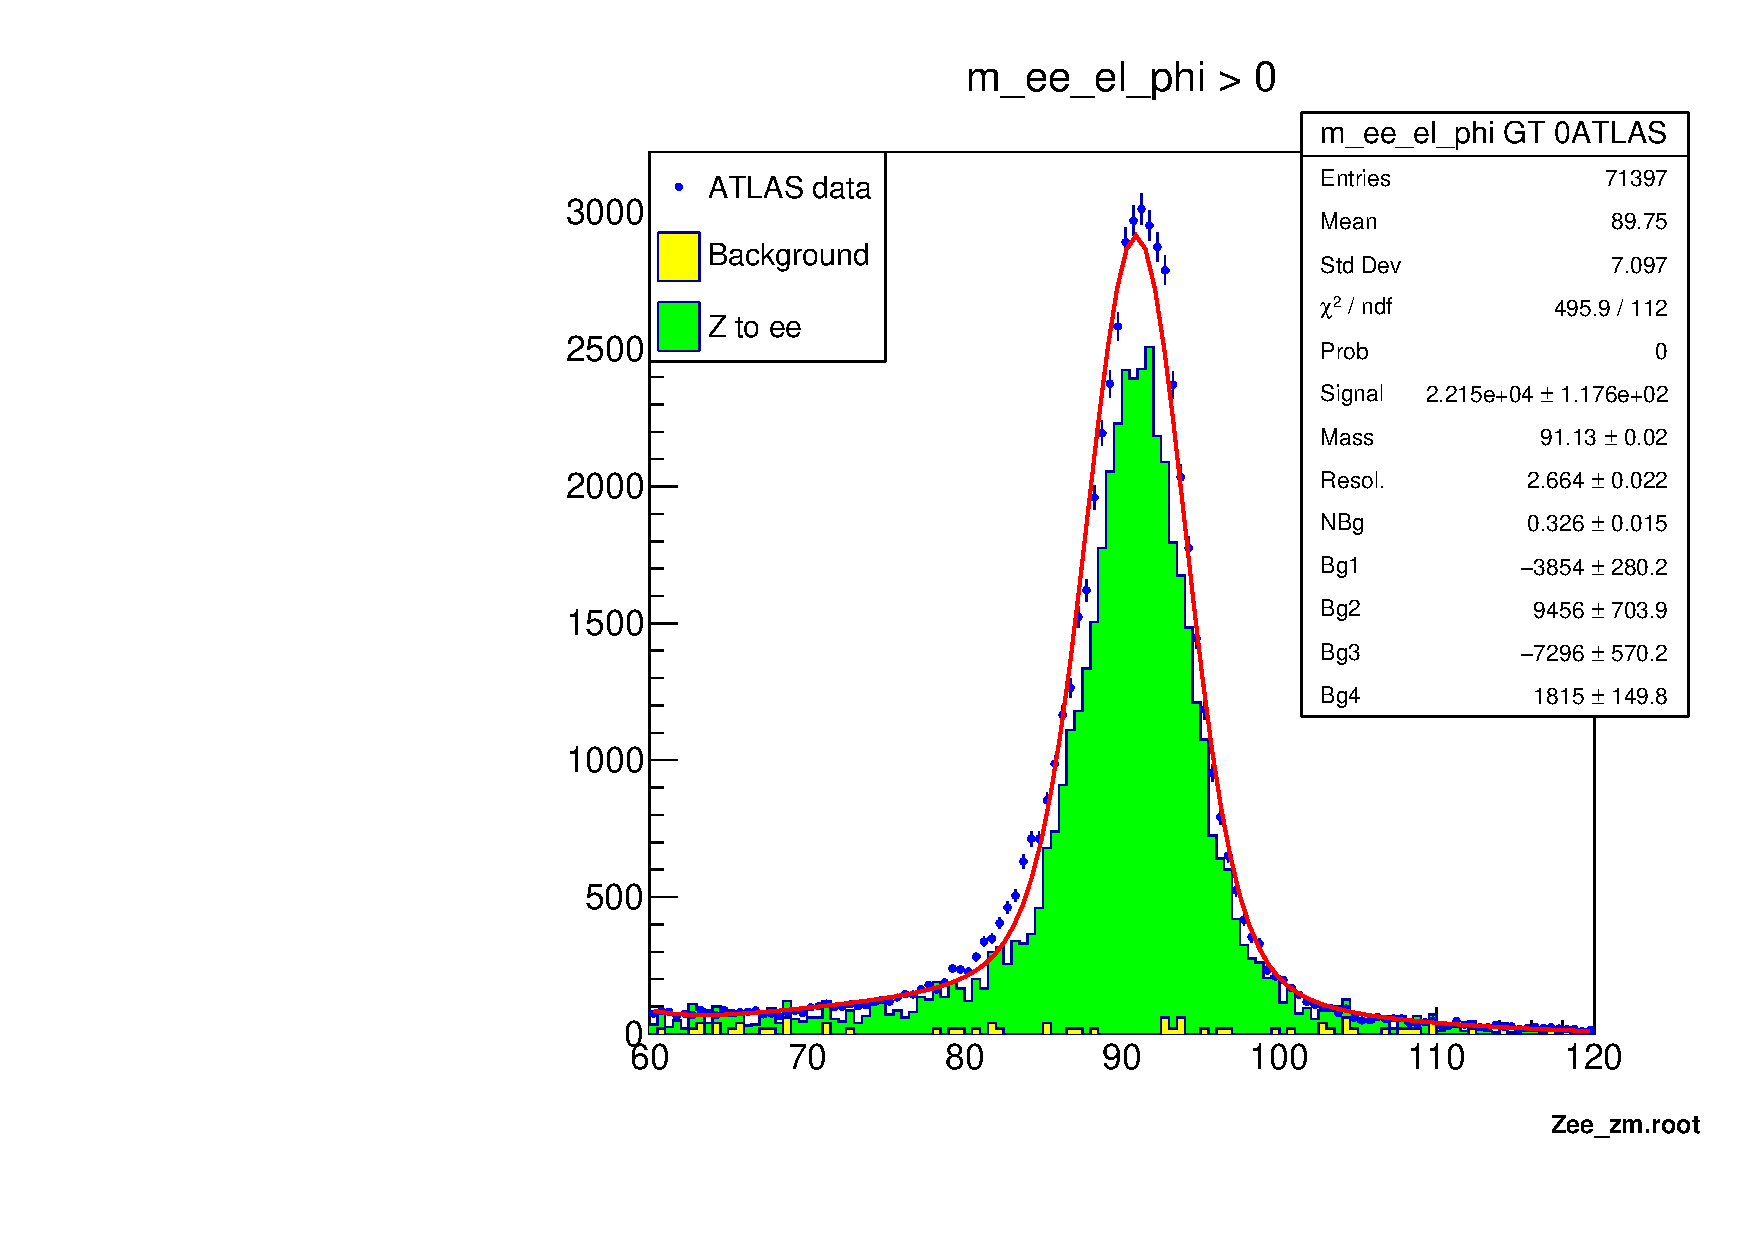
\includegraphics[width=0.7\textwidth]{../W_mass/Z_mass_check_phi_positive.pdf}
        \caption{$Z_mass_check_el_pt-cut.pdf$}
        \label{fig:z-mass_check}
    \end{figure}

    \begin{table}[H]
        \centering
        \begin{tabular}{ccc}
            \toprule
            \toprule
            cut selection & $M_{Z^0,meas}$ / GeV & $\bigl| \frac{M_{Z^0,meas}- M_{Z^0,lit}}{M_{Z^0,meas}} \bigr|$ \\
            \midrule
            $p_{T,e^{\pm}} > 40$ GeV & $91.71 \pm 0.02$ & \\
            $p_{T,e^{\pm}} < 40$ GeV & $90.5 \pm 0.0$ & \\
            $35 < p_{T,e^{\pm}} < 55$ GeV & $91.43 \pm 0.02$ & \\
            $\eta > 2$ & $89.89 \pm 0.05$ & \\
            $\eta < 0.5$ \& $p_{T,e^{\pm}} > 40$ & $91.69 \pm 0.02$ & \\
            $\eta < 0.5$ \& $p_{T,e^{\pm}} < 40$ & $90.56 \pm 0.03$ & \\
            $\phi < 0$ & $91.14 \pm 0.02$ & \\
            $\phi > 0$ & $91.13 \pm 0.02$ & \\
            \bottomrule
            \bottomrule
        \end{tabular}
        \caption{Measured $Z^0$ mass for different cut selections}
        \label{tab:z-masses}
    \end{table}


\subsection{QCD scale factor and Kinematic Variables}
    \label{sec:qcd_factor/variables}
    In order to achieve an accurate measurement of the W-mass, the background processes at ATLAS have to be taken into consideration.
    At LHC, proton proton collisions cause the measured events, therefore the background coming from QCD processes is large. This causes a problem,
    since the final products of the $W \rightarrow e\nu$ events we use to measure the W-mass are leptons which do not interact with the strong interaction.
    This makes the simulation of a QCD background for the $W \rightarrow e\nu$ events difficult. In order to solve this problem, the QCD background is extracted
    from the data. In order to scale the data correctly, a QCD scale factor is used, since the integrated luminosity of the background is not measured and therefore
    unknown. In order to get an understanding of the QCD scale factor and its effect on the data, different kinematic values are be plotted for different 
    QCD scale factors.

\subsubsection{Kinematic Variables}
    \label{sec:variables}
    In order to get a feeling for the QCD scale factor and estimate its optimal value, different kinematic Variables are analyzed.
    The chosen kinematic variables are \texttt{el\_pt} (the transverse momentum of the electron), \texttt{etmis} (missing transverse energy/momentum),
    \texttt{njet} (number of jets in the event) and \texttt{ptw} (transverse momentum of the W boson). The distributions of these different variables
    for a scale factor of 1 (meaning no scaling) can be seen in figure \ref{fig:qcd1}. From figure \ref{fig:qcd1} it is obvious that the ATLAS data does not agree very well with 
    the simulations. In order to solve this, the QCD scale factor was set to different values whilst looking at the distributions until the agreement between real and simulated data
    was optimal by eye. Compromises were necessary, since the alignment between real data and simulated data was unequal for different regions. 
    After some trial and error, the optimal QCD scale factors the four mentioned kinematic variables were chosen as:
    \begin{table}[H]
        \centering
        \begin{tabular}{cc}
            \toprule
            Variable & QCD scale factor \\
            \midrule
            \texttt{etmis}   &  $0.30 \pm 0.05$ \\ 
            \texttt{el\_pt}  &  $0.35 \pm 0.07$ \\
            \texttt{nejt}    &  $0.46 \pm 0.08$ \\
            \texttt{ptw}     &  $0.42 \pm 0.06$ \\
            \bottomrule
        \end{tabular}
        \caption{Optimal QCD scale factors for each of the examined kinematic variables.}
        \label{tab:scale_factors}
    \end{table}
    The errors were chosen to account for the previously mentioned problem, that the data aligned unequally well with the simulated data in different regions of the distributions.
    Therefore the errors were chosen, such that at the end of the error interval, the alignment was best in one region whilst the disalignment in the rest of the distribution was
    still decent. 
    Overall the kinematic variables display the expected behavior. The transverse momentum of the W-boson \texttt{ptw} is mostly small, meaning less than ca. 30\,GeV.
    When looking at the electron transverse momentum \texttt{el\_pt}, the $W \rightarrow e\nu$ events display a peak between 40 and 50\,GeV which is expected since this 
    is around half the mass of the W-boson, which is coming from the Jacobi peak \cite{manual}. The increase towards lower $p_T$ is mostly due to QCD background.
    When looking at the missing transverse momentum \texttt{etmis} the distribution behaves similarly to the electron transverse momentum \texttt{el\_pt}, which is expected.
    Since the transverse momentum of the W-bosons is mostly small, compared to that of the from the decay resulting electron and neutrino, due to momentum conservation, the 
    electron and the neutrino get approximately half the W-boson mass as energy. It is therefore expected that both these distributions, when disregarding the background, 
    feature a peak located around the W-boson mass. The distribution 
    \begin{figure}[H]
        \begin{subfigure}{0.5\textwidth}
            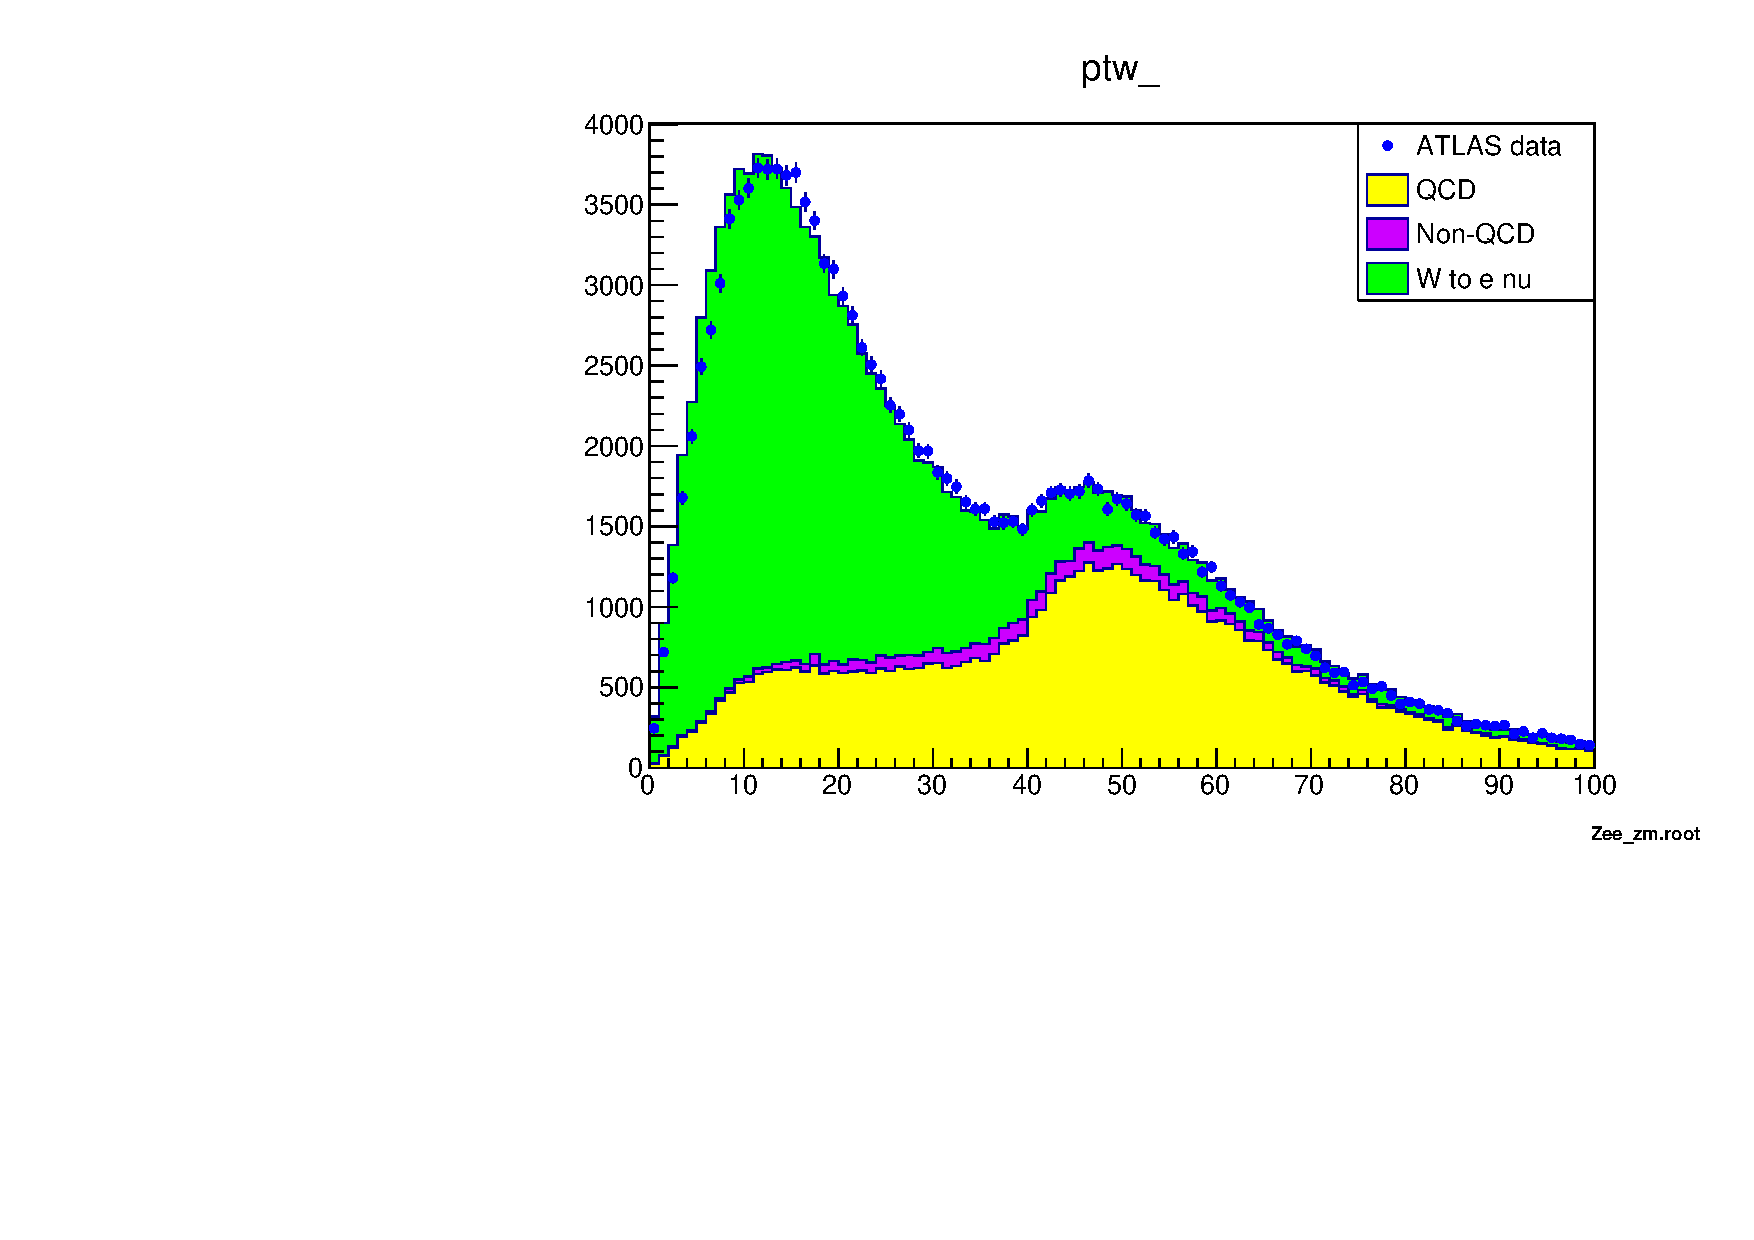
\includegraphics[width=\textwidth]{../W_mass/ptw_100_0_100_qcd0-42.pdf}
        \end{subfigure}
        \begin{subfigure}{0.5\textwidth}
            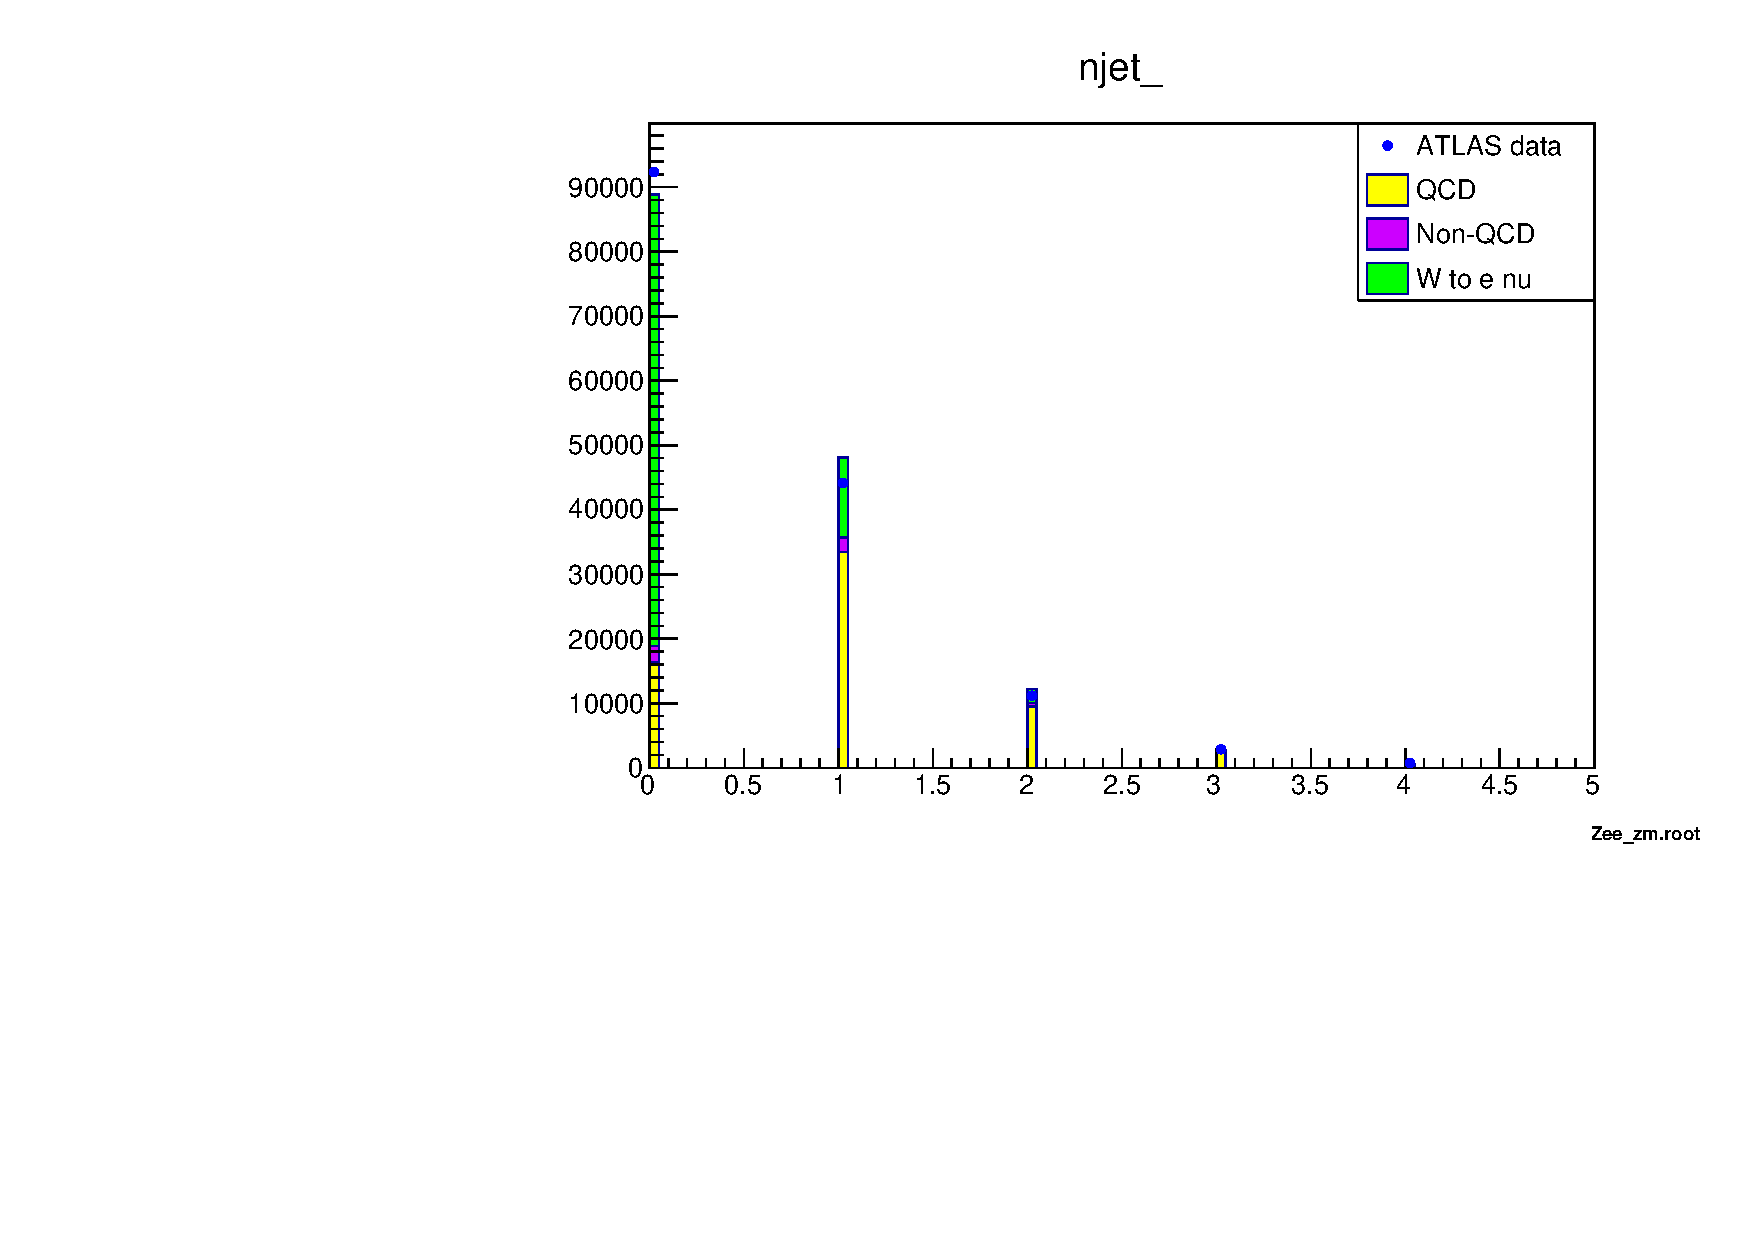
\includegraphics[width=\textwidth]{../W_mass/njet_100_0_5_qcd0-42.pdf}
        \end{subfigure}
        \begin{subfigure}{0.5\textwidth}
            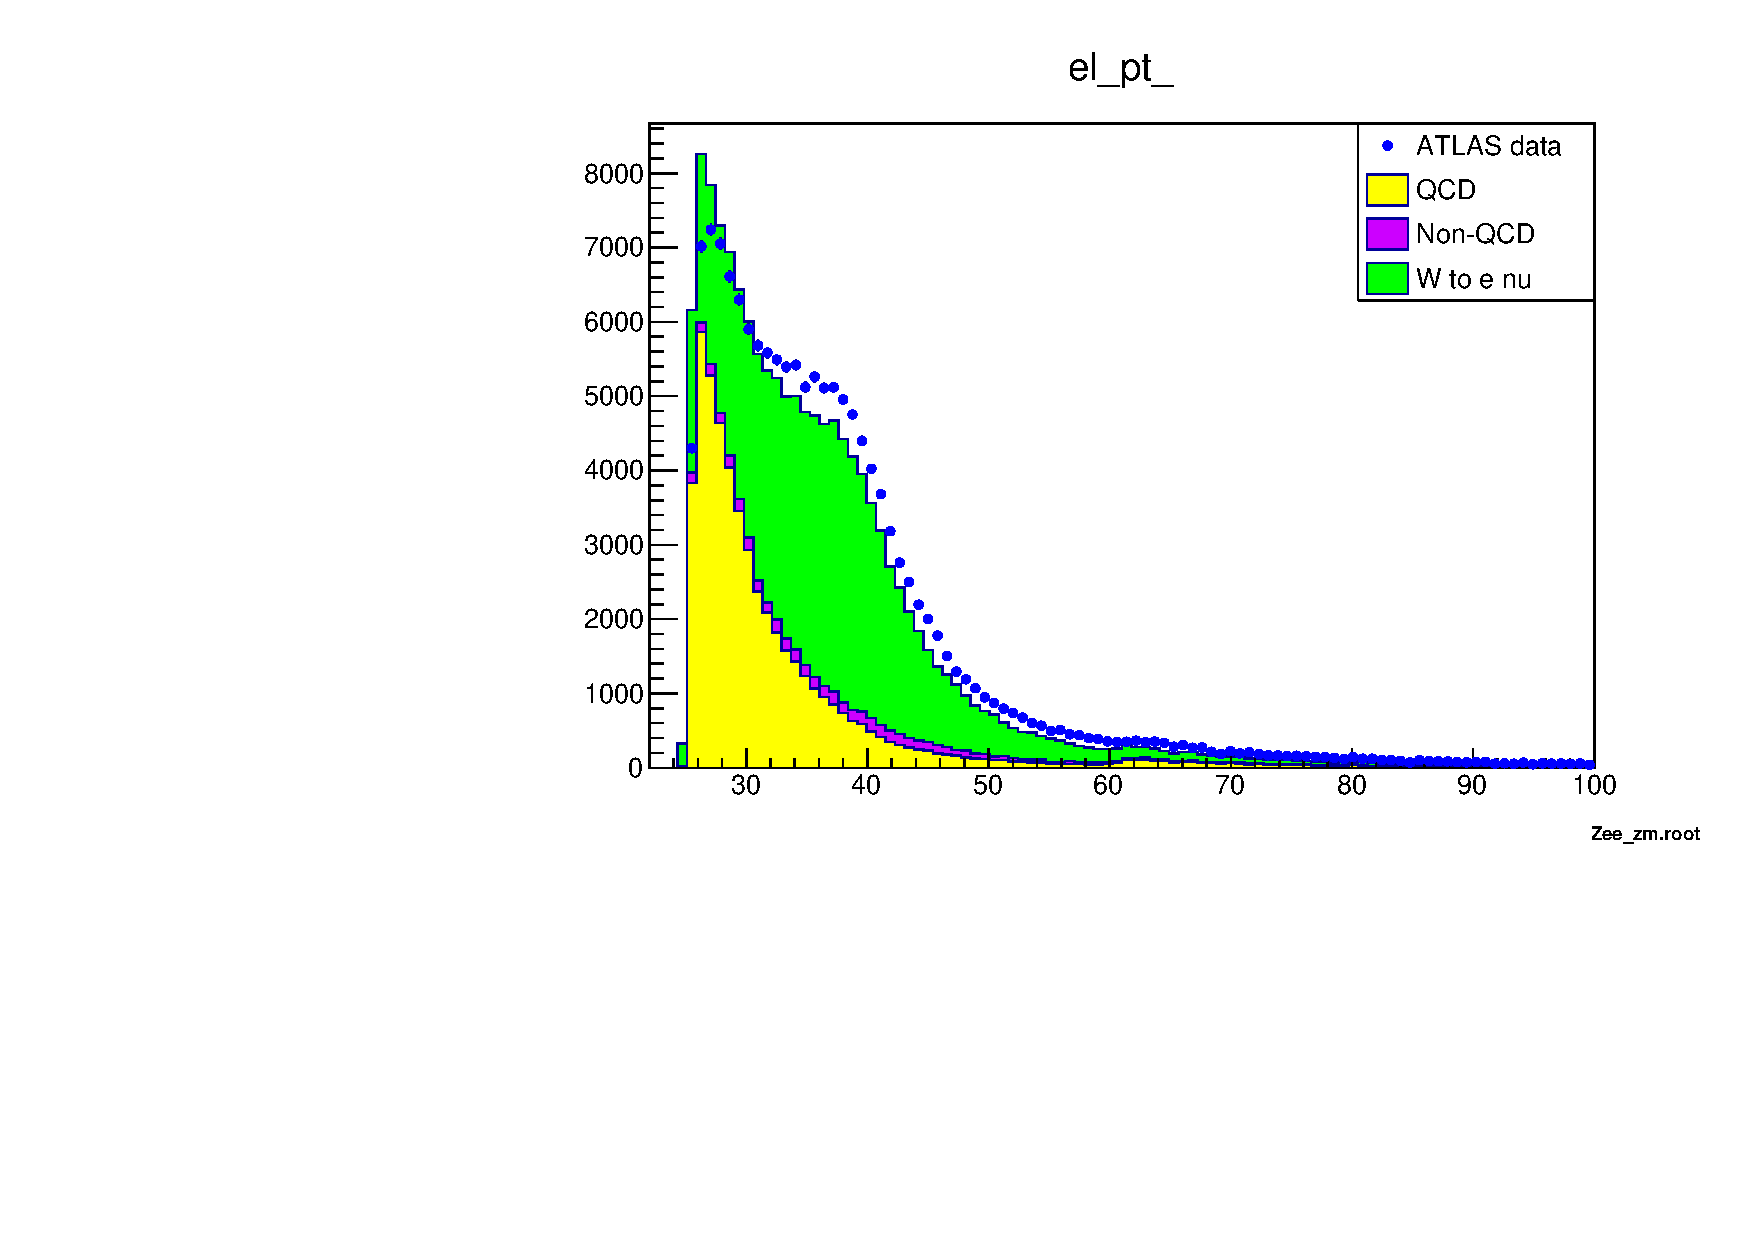
\includegraphics[width=\textwidth]{../W_mass/elpt_100_25_100_qcd0-35.pdf}
        \end{subfigure}
        \begin{subfigure}{0.5\textwidth}
            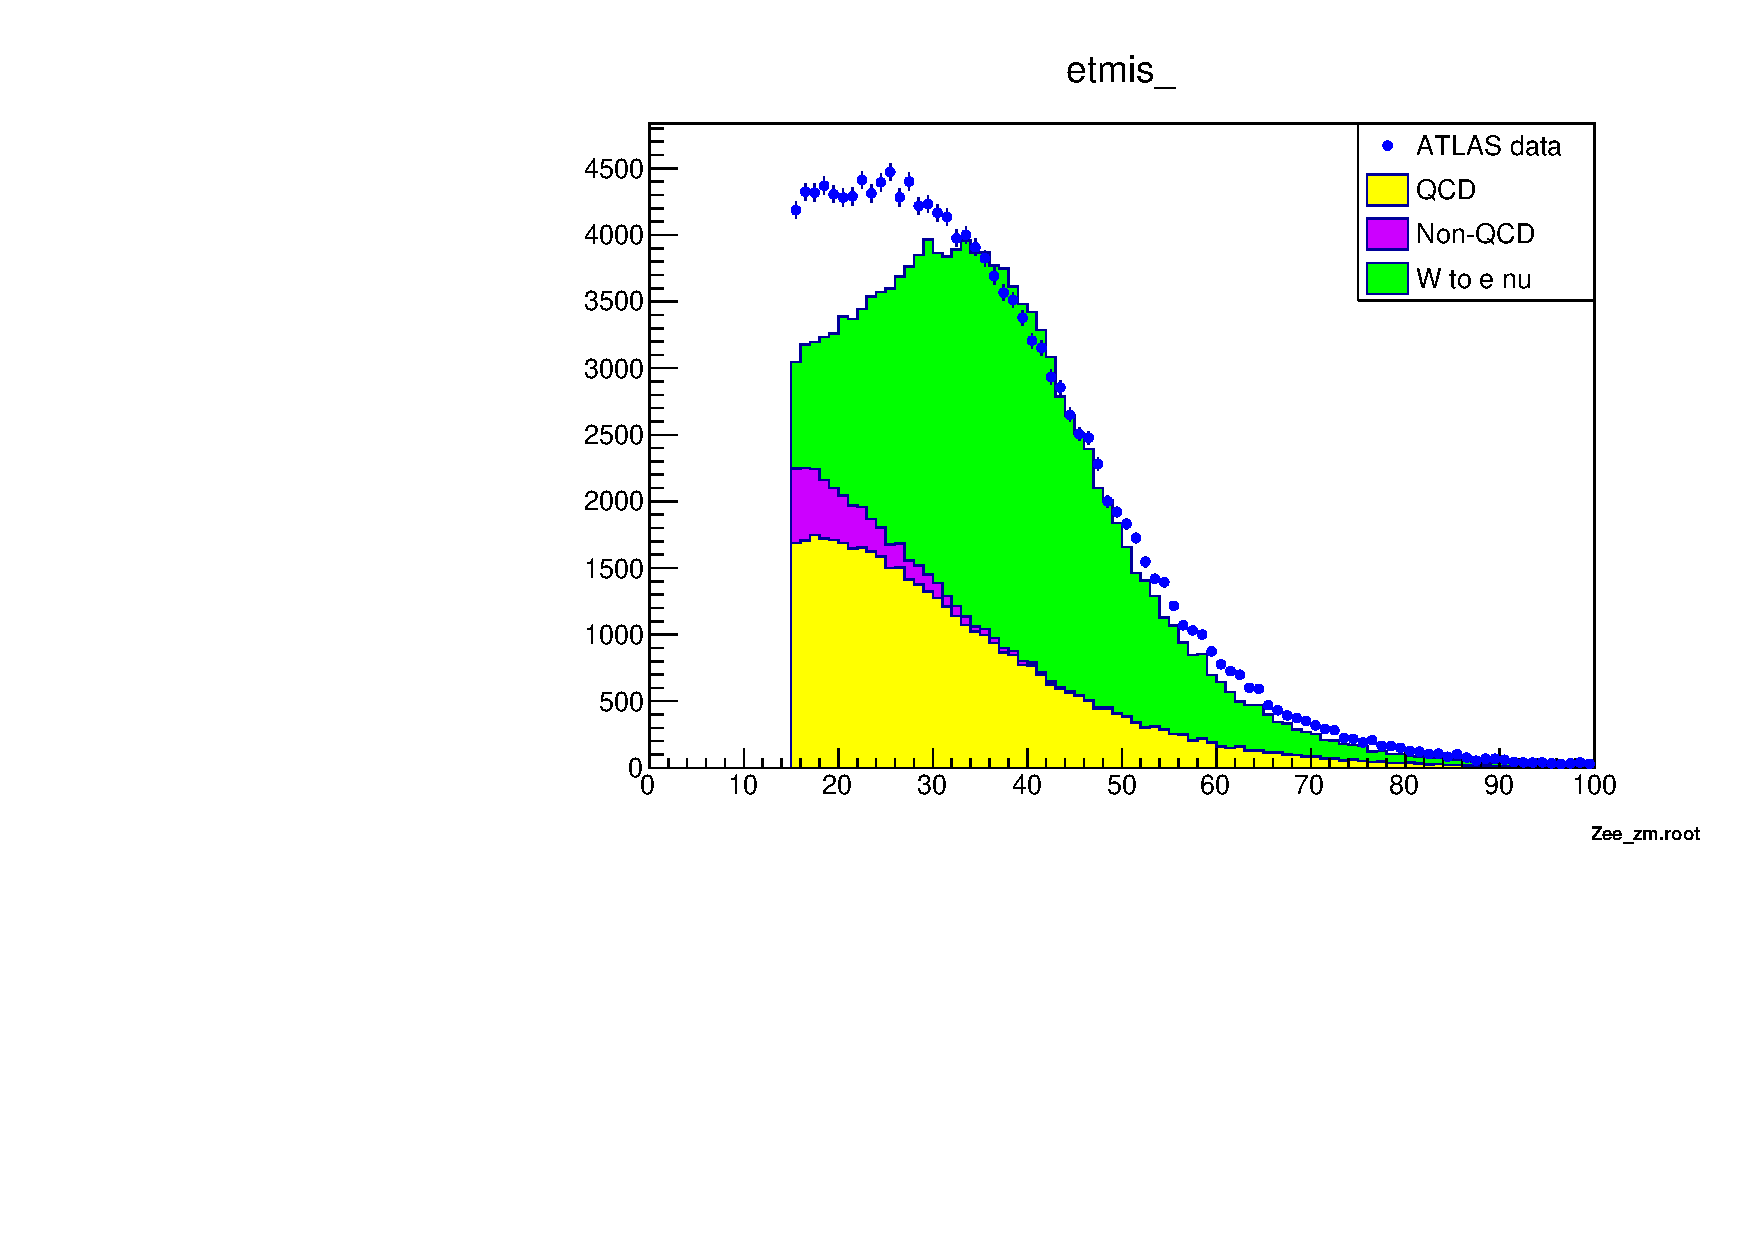
\includegraphics[width=\textwidth]{../W_mass/etmis_100_0_100_qcd0-3.pdf}
        \end{subfigure}
        \caption{Distributions of the kinematic variables \texttt{ptw}, \texttt{njet}, \texttt{el\_pt} and \texttt{etmis} for the QCD factors mentioned in table \ref{tab:scale_factors}}
        \label{fig:qcd-final}
    \end{figure}
    In the next step, the distribution of $p_T^W$ is analyzed for events with different jet multiplicities. The corresponding histograms are displayed in figure \ref{fig:ptw_jets}.
    A clear trend is observed: the signal-to-background ratio decreases as the number of jets increases.
    This behavior aligns with the jet multiplicity distribution shown previously in figure \ref{fig:qcd-final}.

    For events with zero jets, the signal is dominant at low $p_T^W$, peaking around 10-15\,GeV. This is expected, as there are no jets present to impart recoil to the W boson.
    However, when considering events with one jet, the signal drops significantly, and the previously observed peak at low $p_T^W$ disappears.
    Instead, the signal appears relatively flat in the low to mid-$p_T^W$ range and then declines at higher values.
    This can be explained by the presence of one jet in these signal events, which imparts recoil to the W boson.
    Although the jet direction is unknown, assuming an isotropic distribution, this results in a roughly uniform $p_T^W$ distribution.
    Lower $p_T^W$ values correspond to a forward jet recoil, while mid to high $p_T^W$ suggests more transverse recoil.

    The background shows a noticeable increase around 50\,GeVGeV. This could be related to the W boson mass, as the peak occurs slightly above half its mass,
    although other factors may also contribute.

    As the number of jets increases further, the signal continues to diminish while the background becomes more dominant.
    The background still peaks around 50\,GeV, but the overall number of events decreases.
    This trend is consistent with expectations: the original process does not favor the presence of jets,
    and the likelihood of additional (radiated) jets decreases with increasing event complexity, due to a reduction in available vertices.
    \begin{figure}[H]
        \begin{subfigure}{0.5\textwidth}
            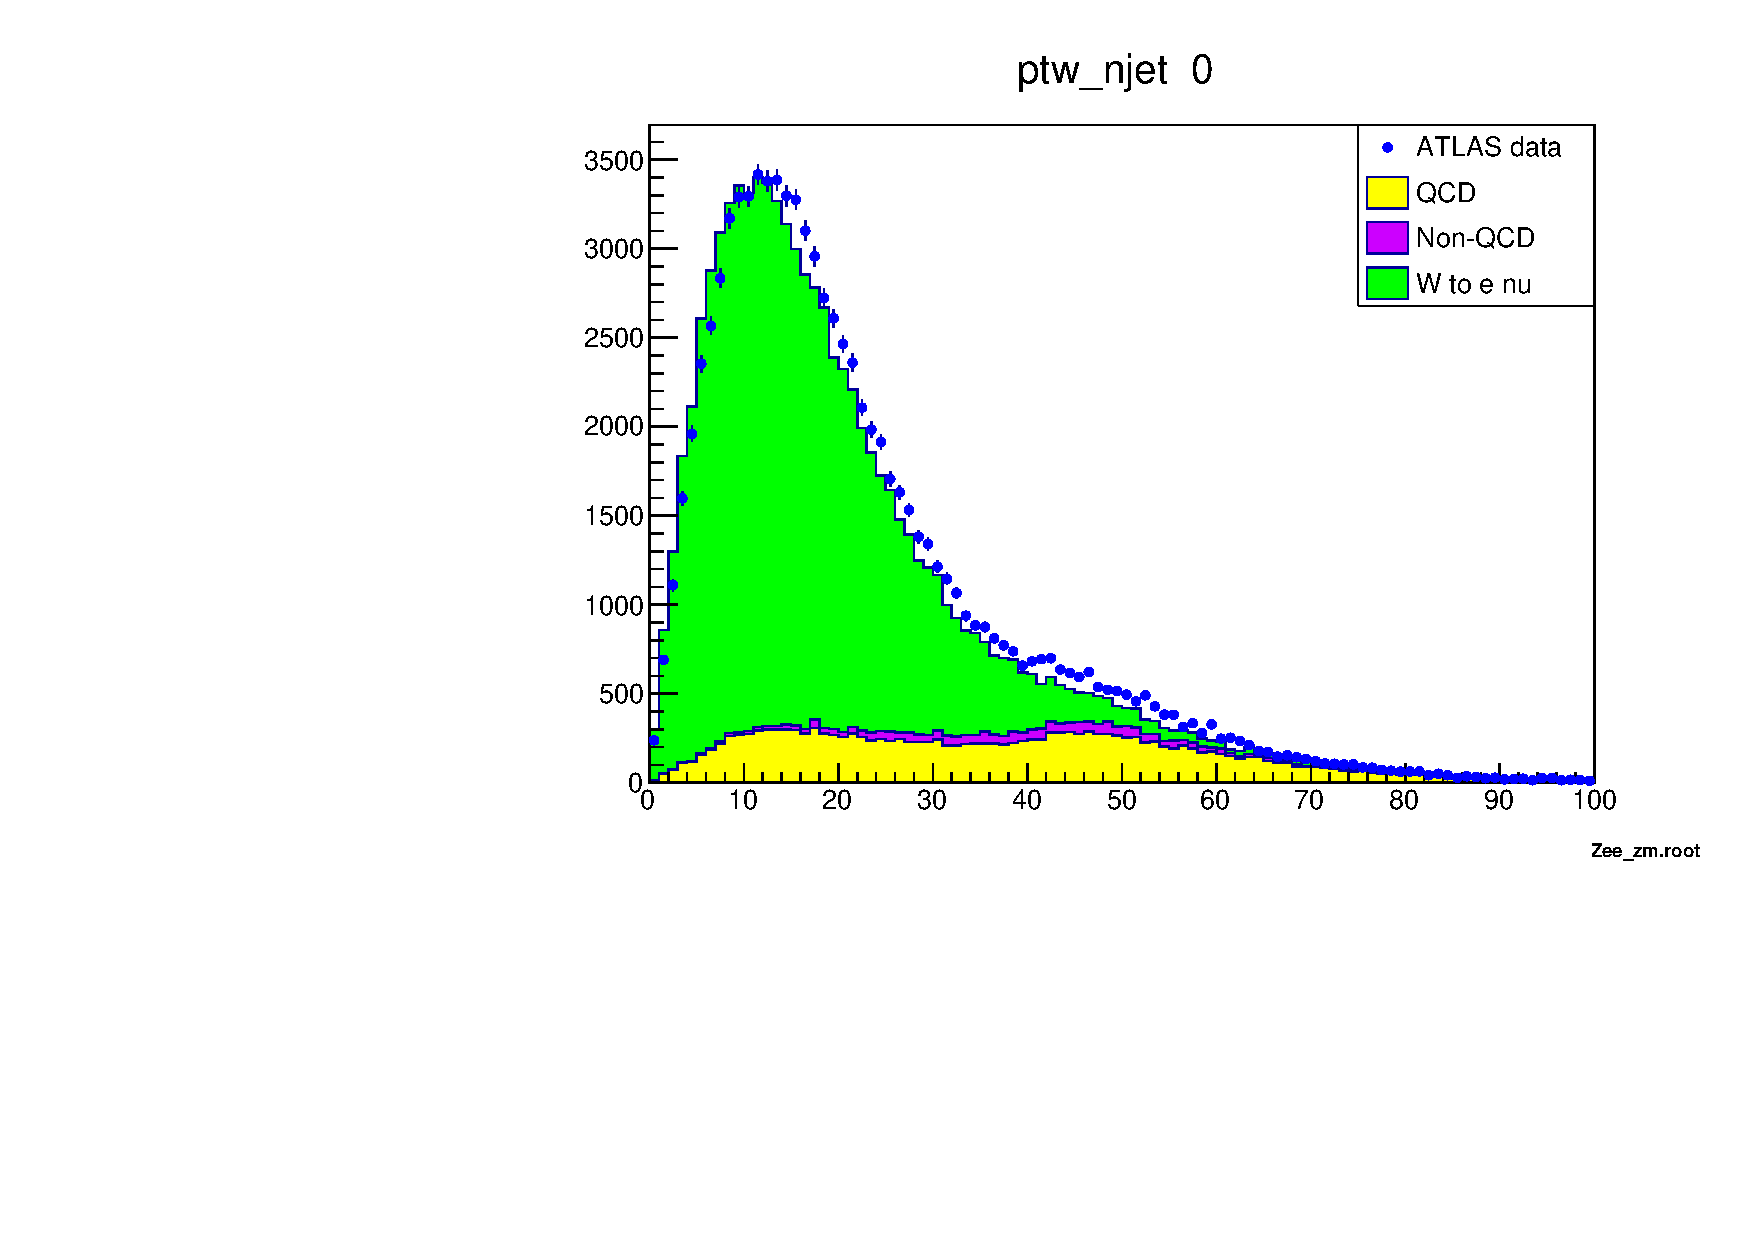
\includegraphics[width=\textwidth]{../W_mass/ptw_njet0.pdf}
            \subcaption{0 jets}
        \end{subfigure}
        \begin{subfigure}{0.5\textwidth}
            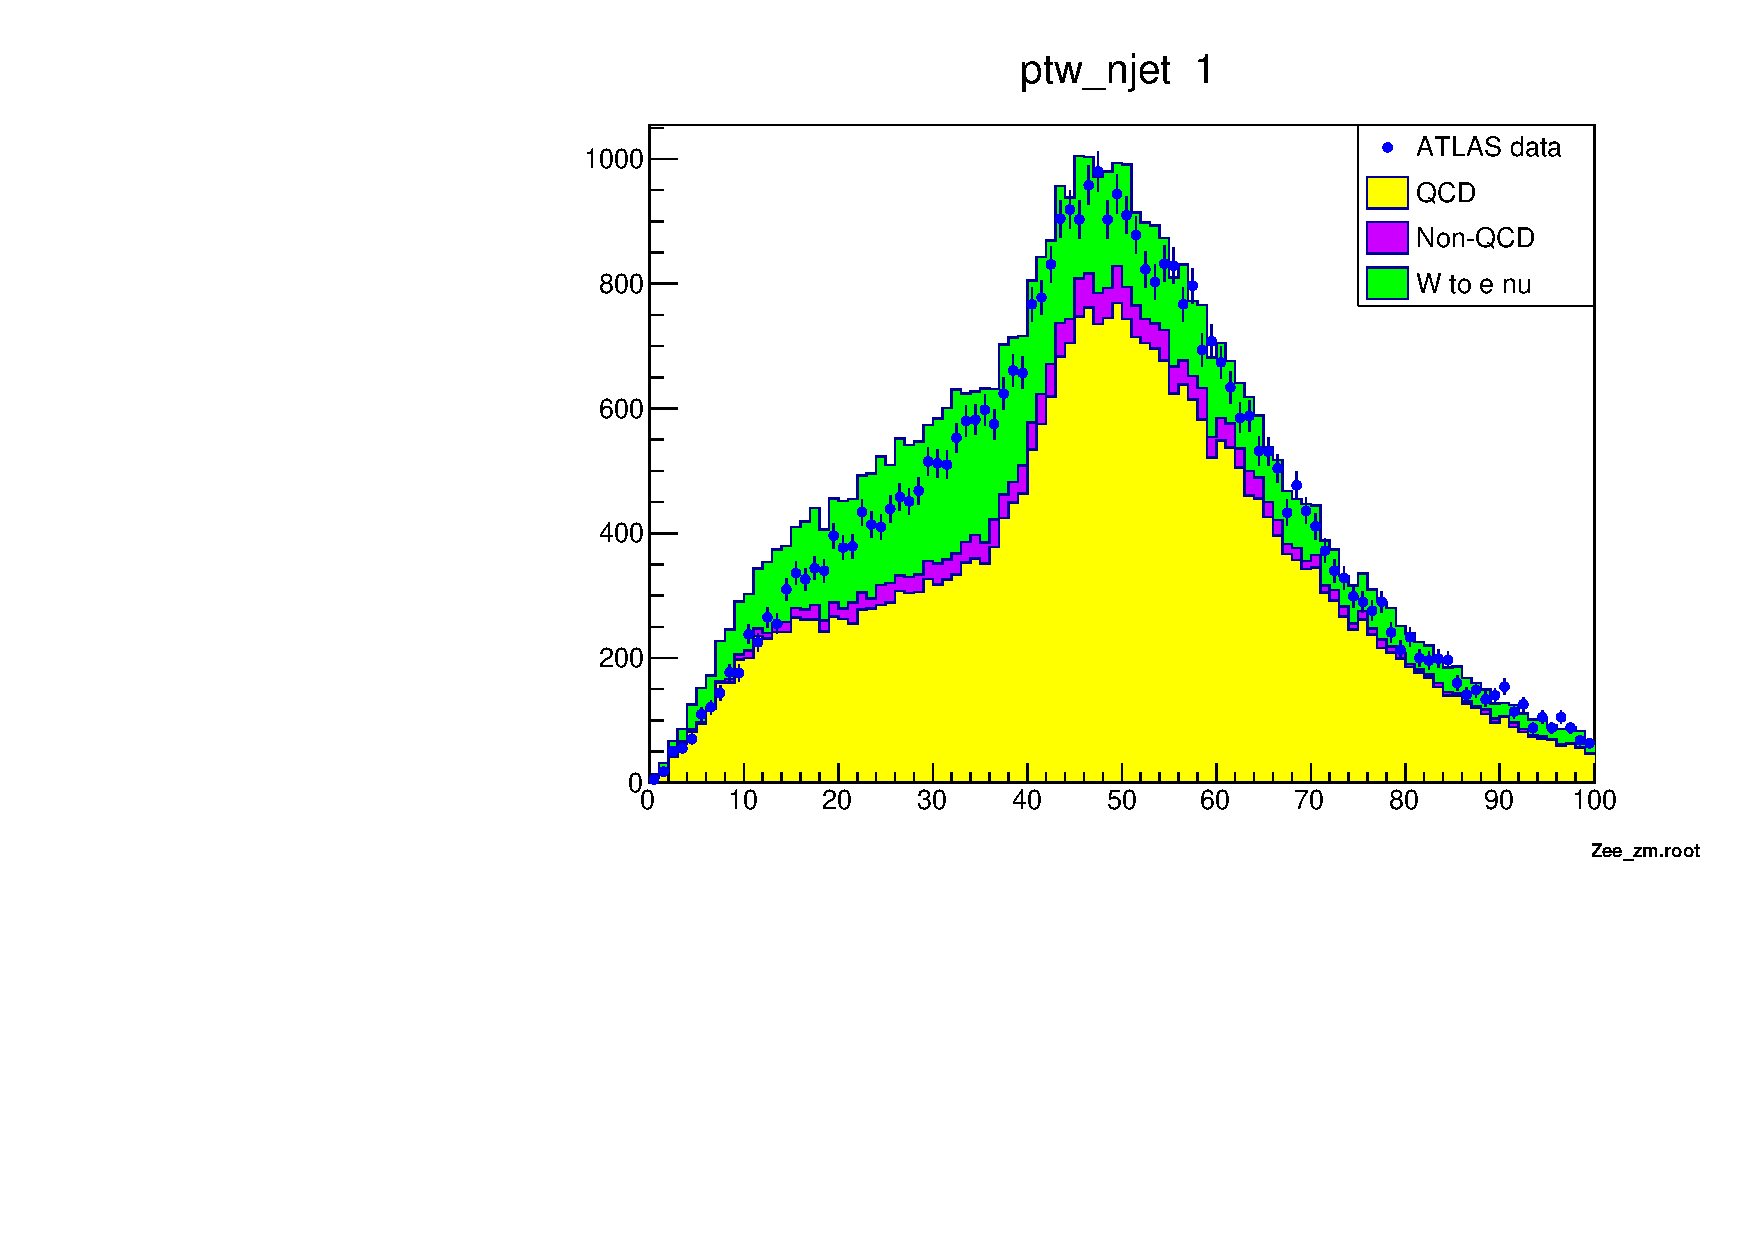
\includegraphics[width=\textwidth]{../W_mass/ptw_njet1.pdf}
            \subcaption{1 jet}
        \end{subfigure}
        \begin{subfigure}{0.5\textwidth}
            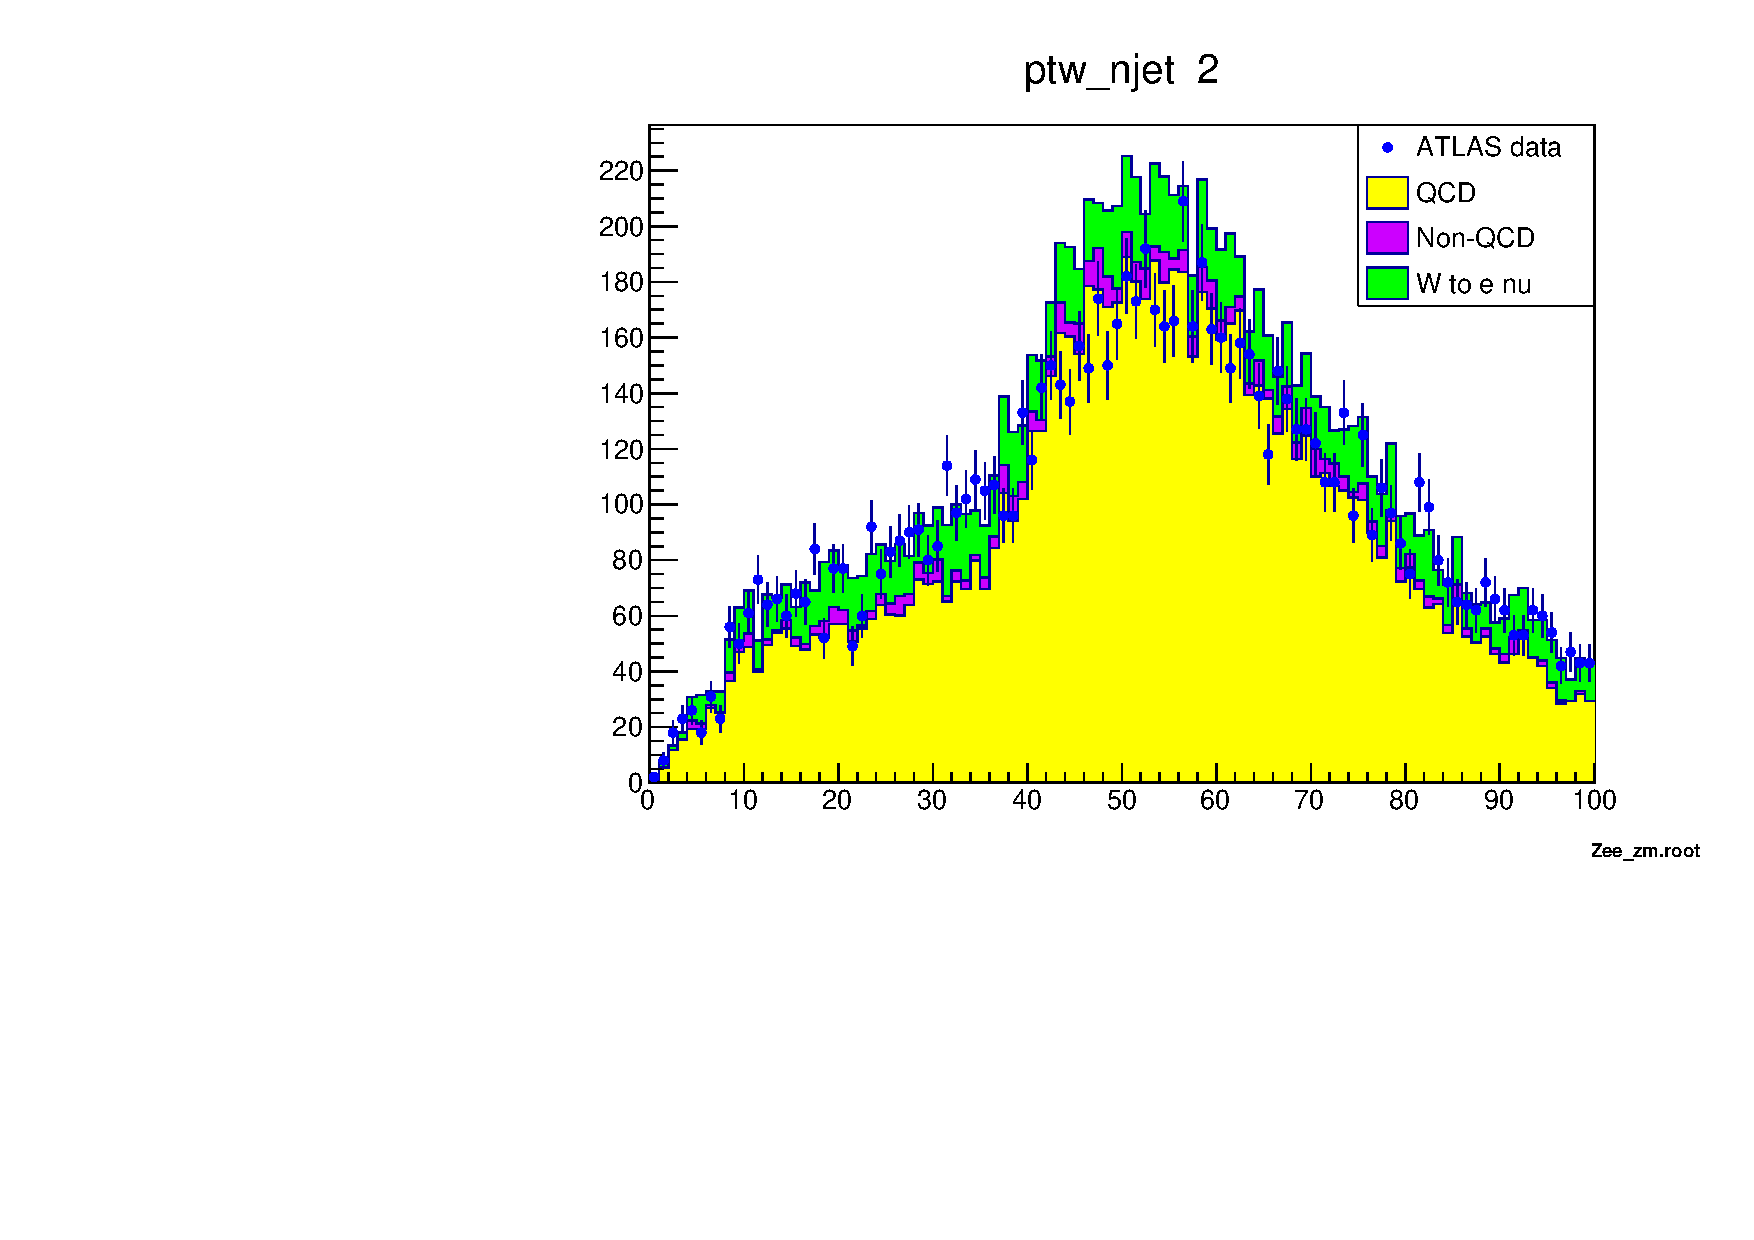
\includegraphics[width=\textwidth]{../W_mass/ptw_njet2.pdf}
            \subcaption{2 jets}
        \end{subfigure}
        \begin{subfigure}{0.5\textwidth}
            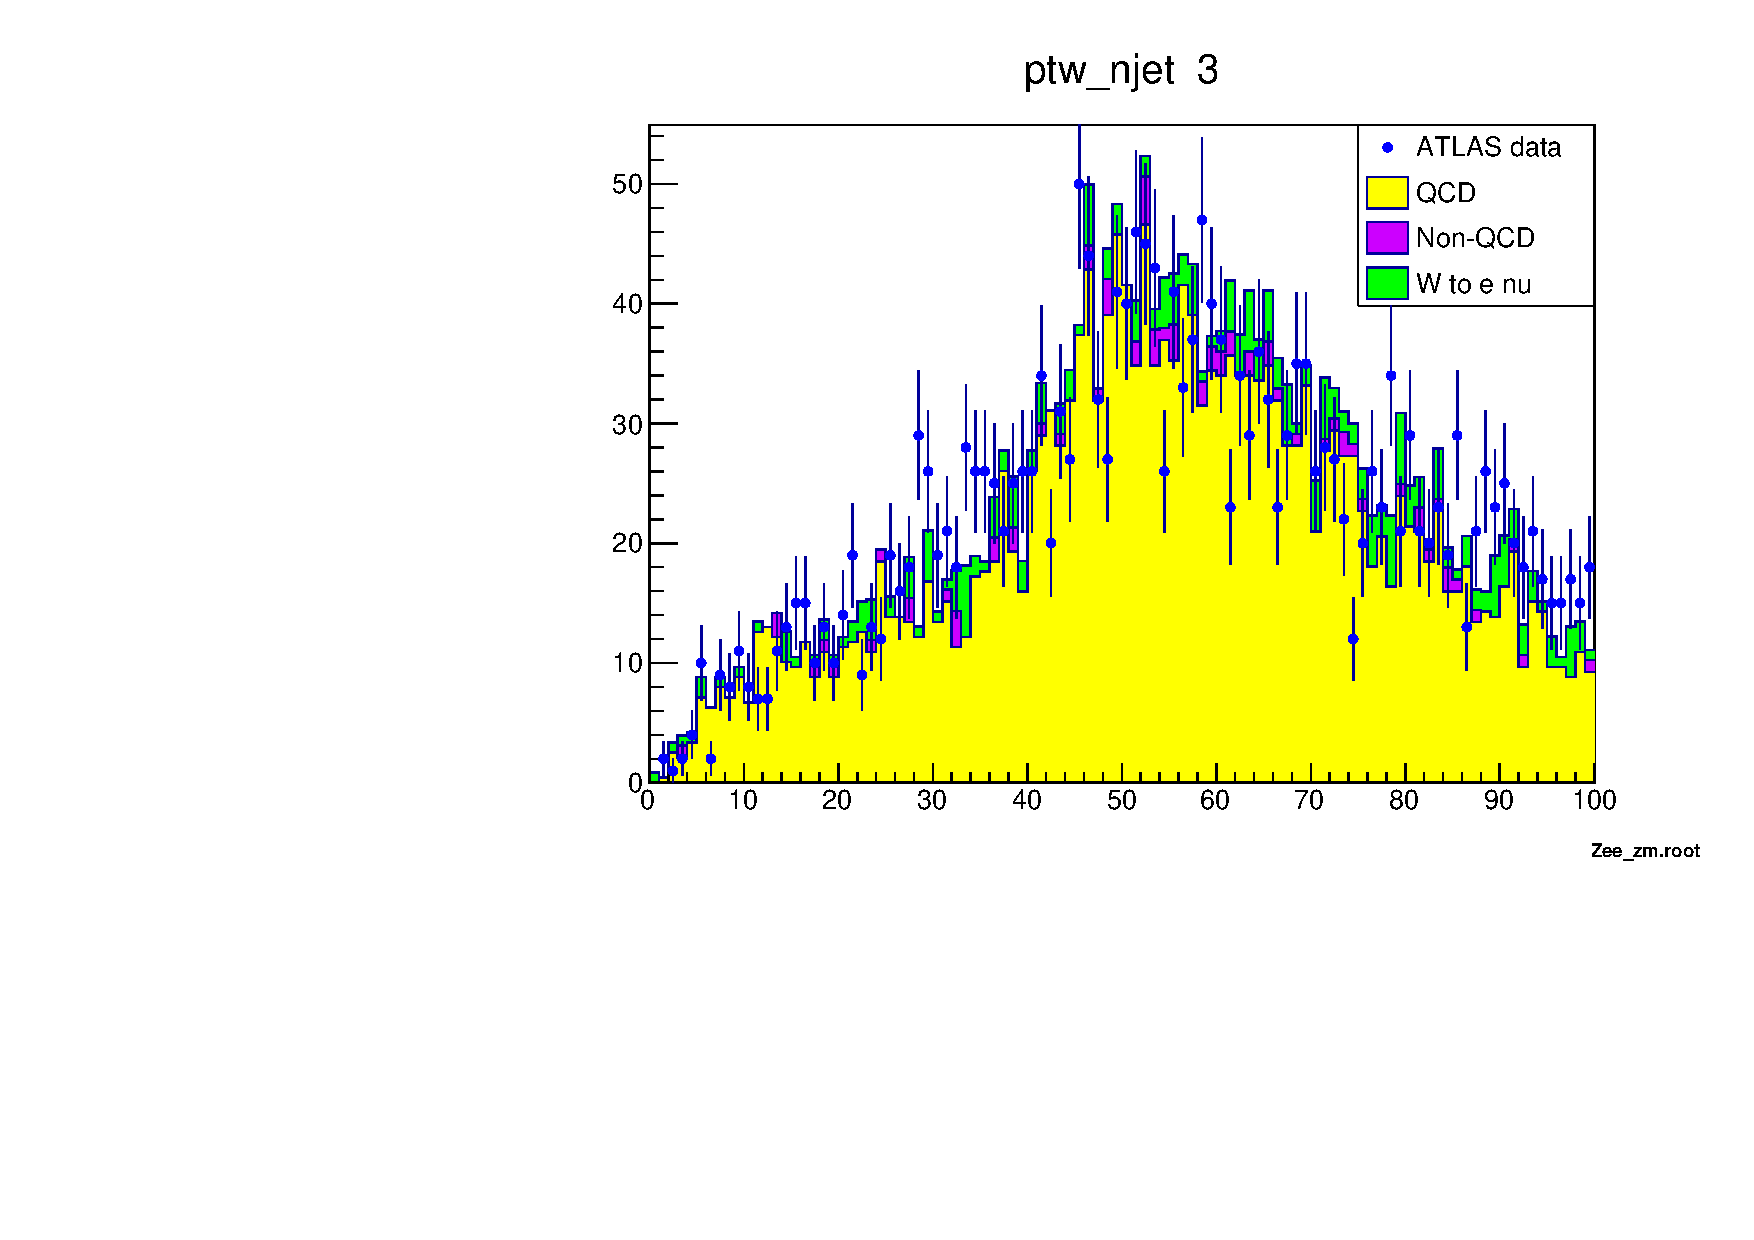
\includegraphics[width=\textwidth]{../W_mass/ptw_njet3.pdf}
            \subcaption{3 jets}
        \end{subfigure}
        \begin{subfigure}{0.5\textwidth}
            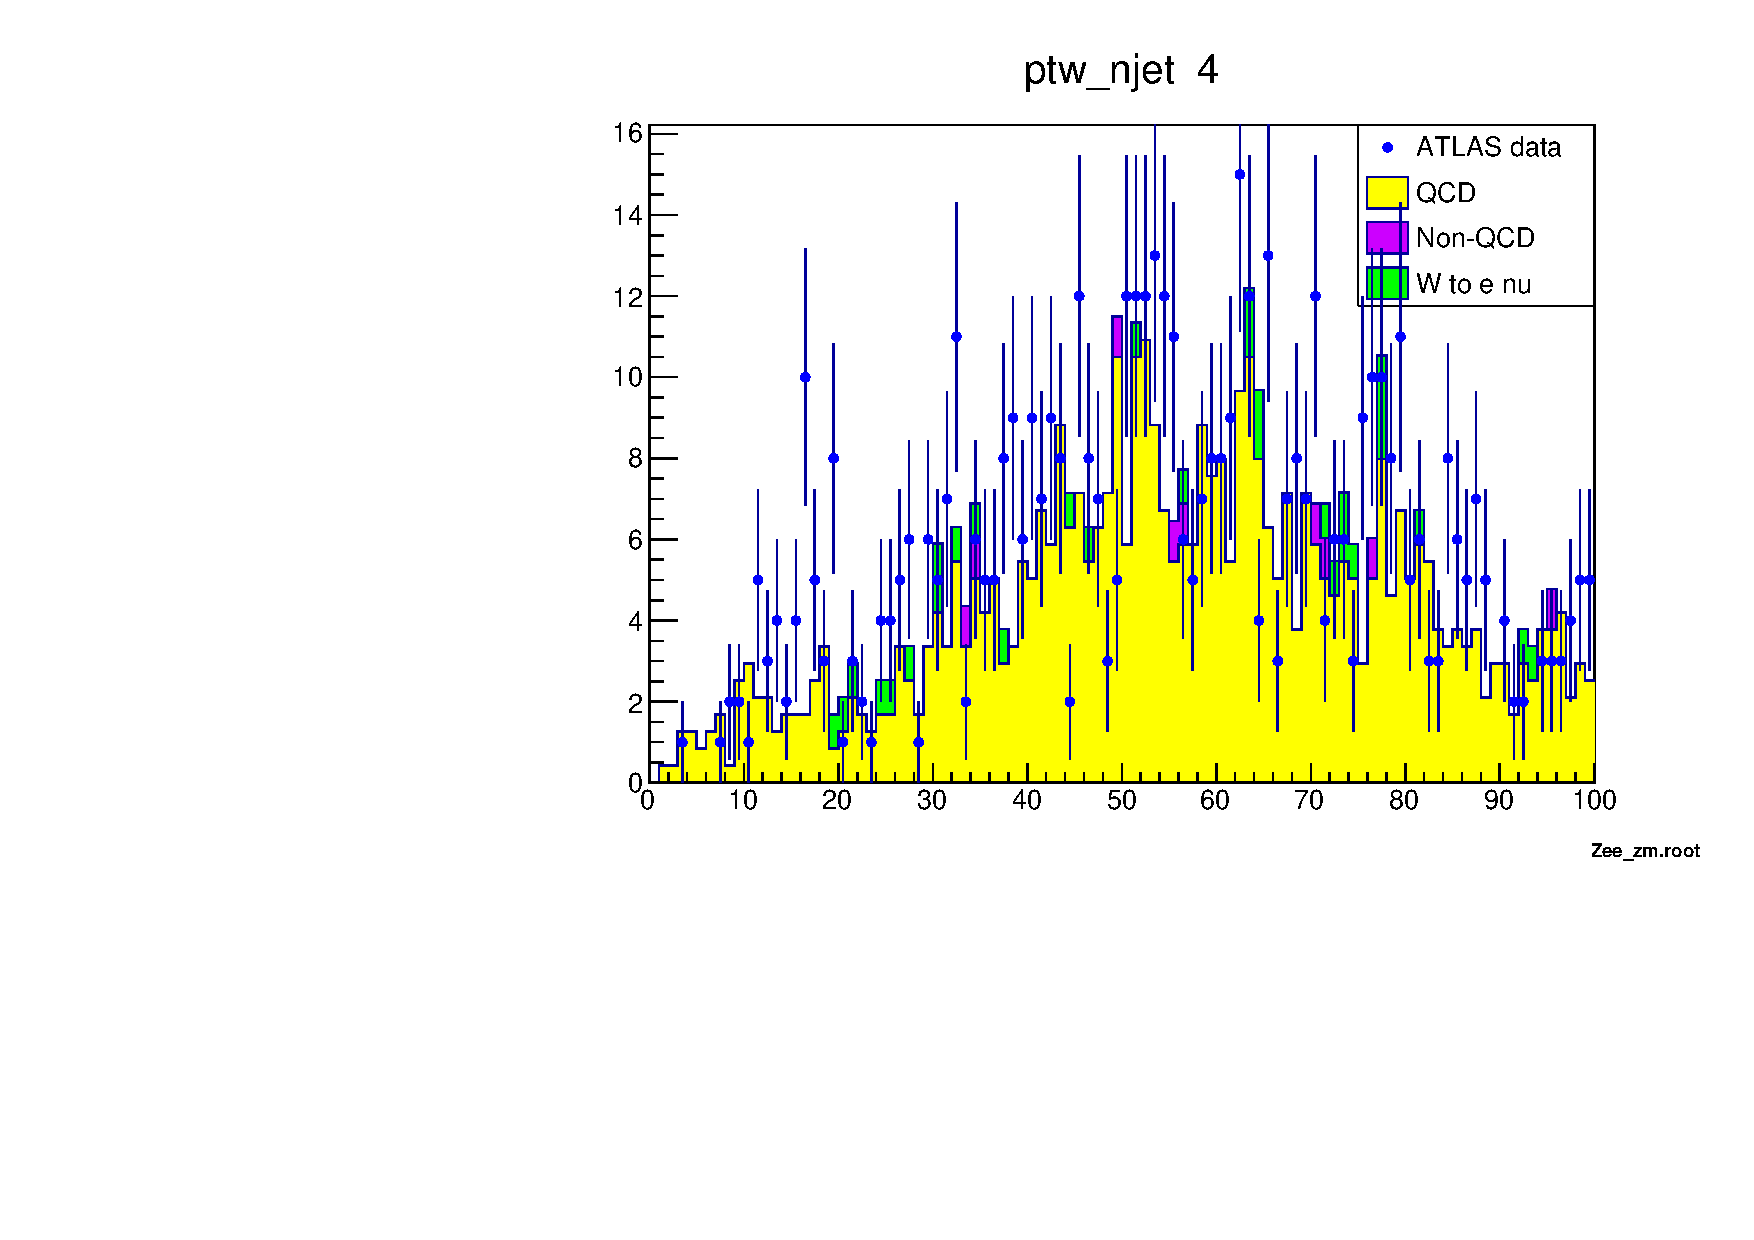
\includegraphics[width=\textwidth]{../W_mass/ptw_njet4.pdf}
            \subcaption{4 jets}
        \end{subfigure}
        \caption{\texttt{ptw} distributions for different number of jets measured in the events}
        \label{fig:ptw_jets}
    \end{figure}
    
\subsubsection{Final QCD scale factor}
    \label{sec:final_qcd}
    After examining the different kinematic variables, a final QCD scale factor has to be chosen. 




\subsection{Cut selection}

\subsection{Gauge curves}

\subsection{W-mass }
